\section{Method}

The initial research phase consisted of a literature study of evolutionary computing in general and then focused on differential evolution, particle swarm optimization and estimation of distribution algorithms, the purpose of which was to understand the state of the art in evolutionary computing and gain the necessary knowledge to evaluate different evolutionary methods and create a new improved algorithm.

\subsection{Tools and environments}

Matlab was used to program all algorithms, benchmark-functions and test-cases. Matlab's neural network package facilitated the testing of neural networks. All graphs we're drawn using Matlab's plotting functions.

\subsection{Benchmarking functions}

The functions for the benchmark are taken from the 2005 CEC conference on continuous evolutionary optimization \cite{suganthan2005problem}. The functions are losely based on the popular optimization benchmark suite created by DeJong \cite{Whitley1996245}.

For all functions $x=[x_1,x_2,x_3,...,x_D]$ are the input parameters, $o=[o_1,o_2,o_3,...,o_D]$ is the global optimum, $D$ is the dimension and $M$ is an orthogonal matrix with parameters unique to each function. The matrices for $o$ and $M$ are available in appendix A. Illustrations of the functions can be found in figures \ref{f1}, \ref{f2}, \ref{f3}, \ref{f4}, \ref{f5}, \ref{f6}, \ref{f7}, \ref{f8}, \ref{f9} and \ref{f10}.

\subsubsection{$F_1$: Shifted Sphere Function}

\begin{equation}
  F_1(x)=\sum_{i=1}^{D}{z_i^2}
\end{equation}
\[ z=x-o \]
\[ x \in [-100,100]^D \]

\begin{figure}[H]
  \centering
  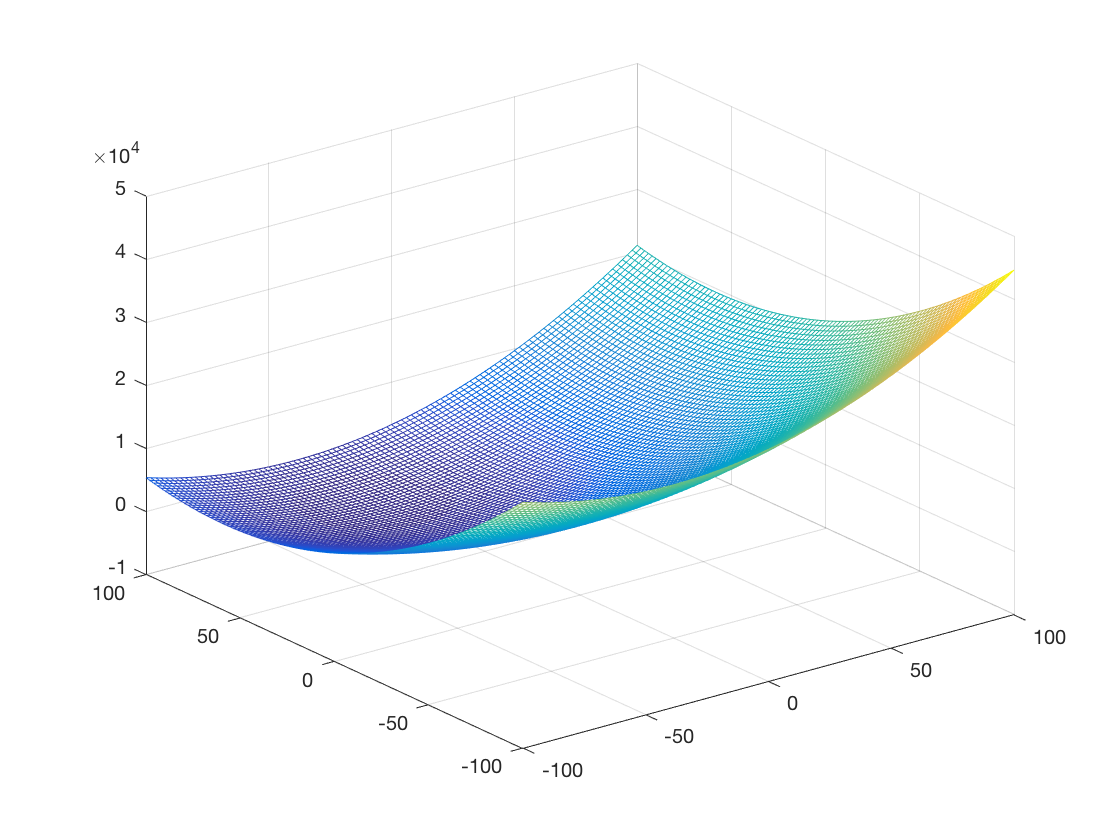
\includegraphics[width=.5\linewidth]{f1}
  \caption{3-D map for 2-D function}
  \label{f1}
\end{figure}

\subsubsection{$F_2$: Shifted Schwefel’s Problem}

\begin{equation}
  F_2(x)=\sum_{i=1}^{D}{(\sum_{j=1}^{i}{z_j})^2}
\end{equation}
\[ z=x-o \]
\[ x \in [-100,100]^D \]

\begin{figure}[H]
  \centering
  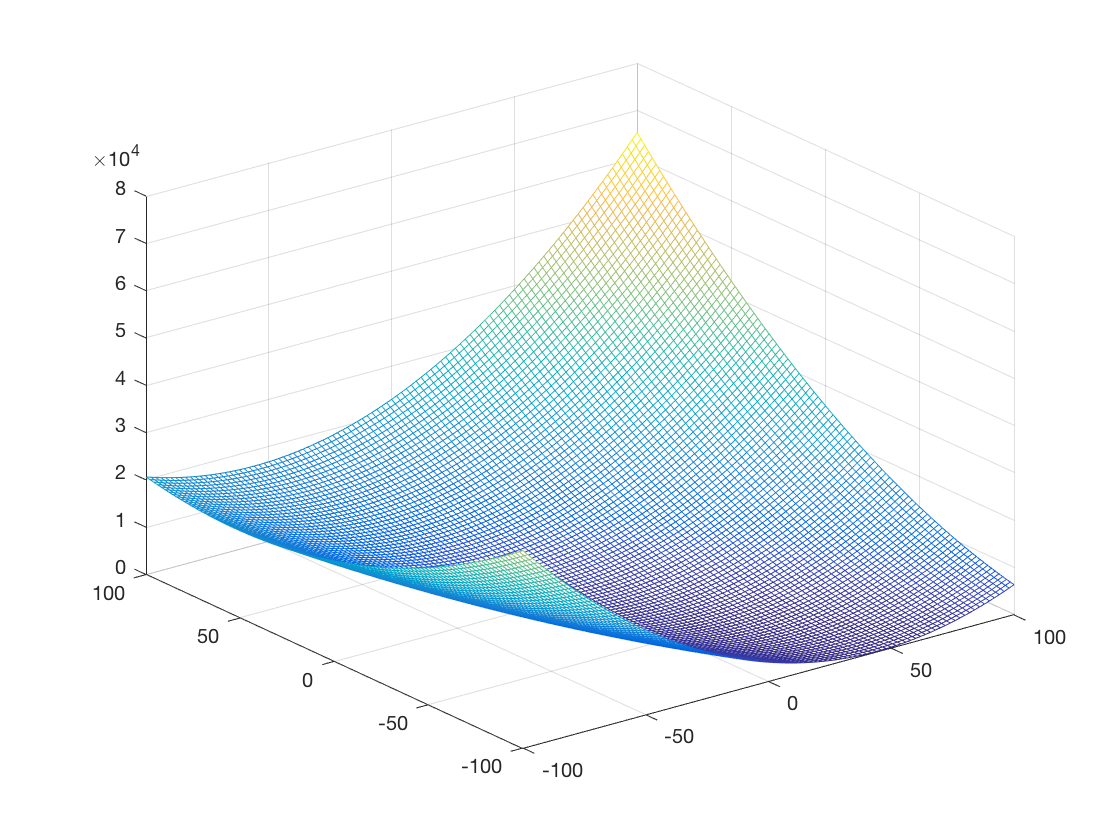
\includegraphics[width=.5\linewidth]{f2}
  \caption{3-D map for 2-D function}
  \label{f2}
\end{figure}

\subsubsection{$F_3$: Shifted Rotated High Conditioned Elliptic Function}

\begin{equation}
  F_3(x)=\sum_{i=1}^{D}{(10^6)^{\frac{i-1}{D-1}}z_i^2}
\end{equation}
\[ z=(x-o)*M \]
\[ x \in [-100,100]^D \]

\begin{figure}[H]
  \centering
  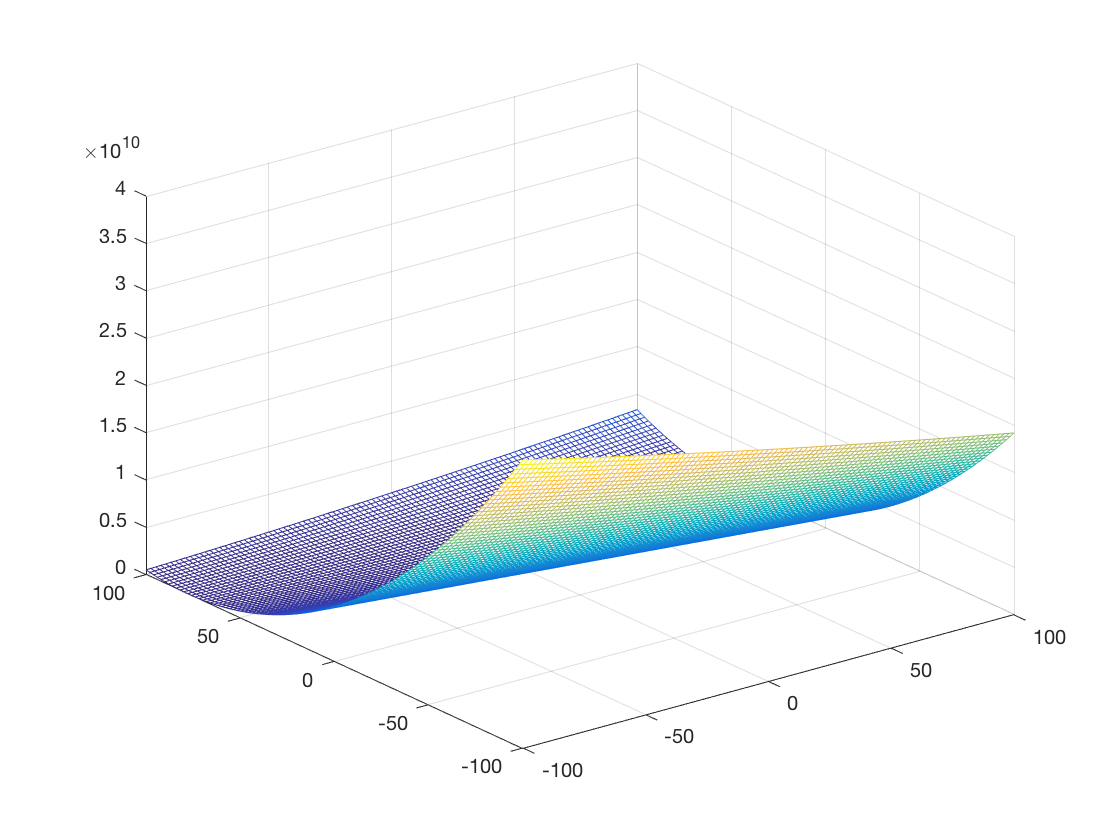
\includegraphics[width=.5\linewidth]{f3}
  \caption{3-D map for 2-D function}
  \label{f3}
\end{figure}

\subsubsection{$F_4$: Shifted Schwefel’s Problem with Noise in Fitness}

\begin{equation}
  F_4(x)=(\sum_{i=1}^{D}{(\sum_{j=1}^{i}{z_j})^2})*(1+0.4|N(0,1)|)
\end{equation}
\[ z=x-o \]
\[ x \in [-100,100]^D \]

\begin{figure}[H]
  \centering
  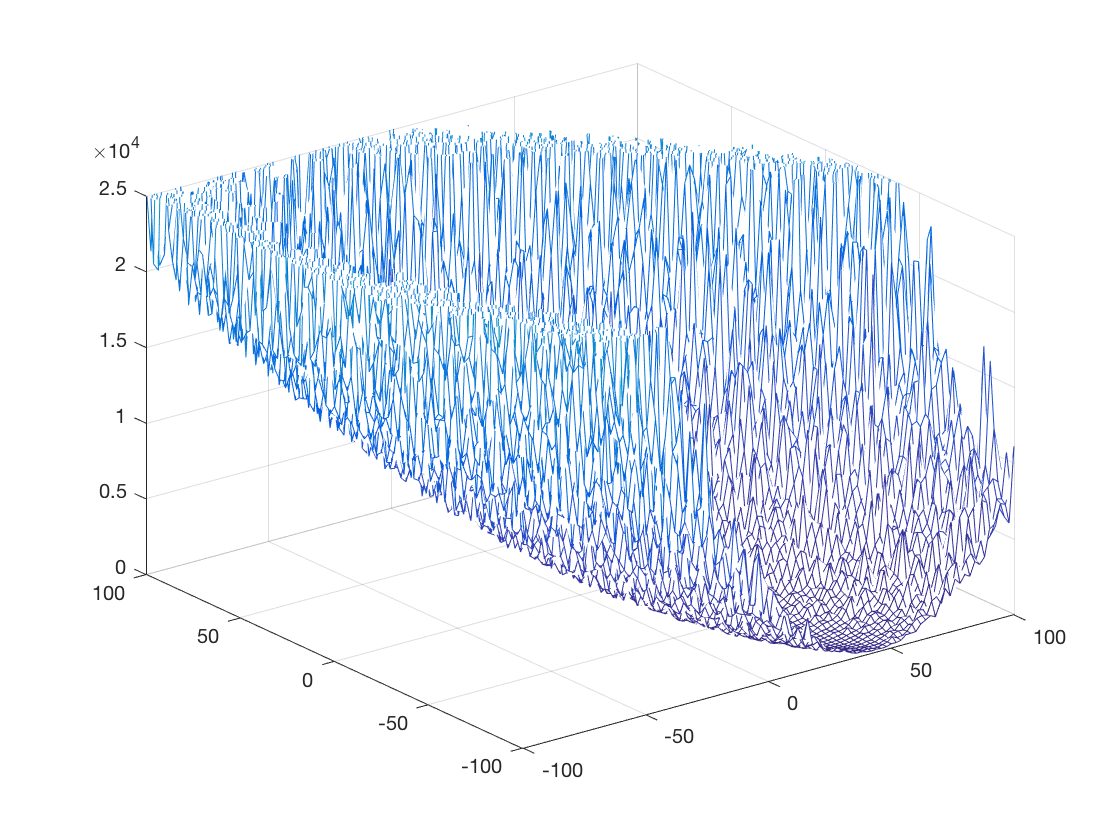
\includegraphics[width=.5\linewidth]{f4}
  \caption{3-D map for 2-D function}
  \label{f4}
\end{figure}

\subsubsection{$F_5$: Schwefel’s Problem with Global Optimum on Bounds}

\begin{equation}
  F_5(x)=max\{|A_ix-B_i|\}
\end{equation}
\[ i=1,...,D, x \in [-100,100]^D \]
\[ A \text{ is a } D*D \text{ matrix}, a_{ij} = \text{ random numbers in } [-500,500],  det(A) \neq 0 \]
\[ B_i = A_i * o, o_i = \text{ random numbers in } [-100,100] \]
\[ o_i = -100 \text{, for } i=1,2,...,[D/4], o_i = 100 \text{, for } i=[3D/4],...,D \]

\begin{figure}[H]
  \centering
  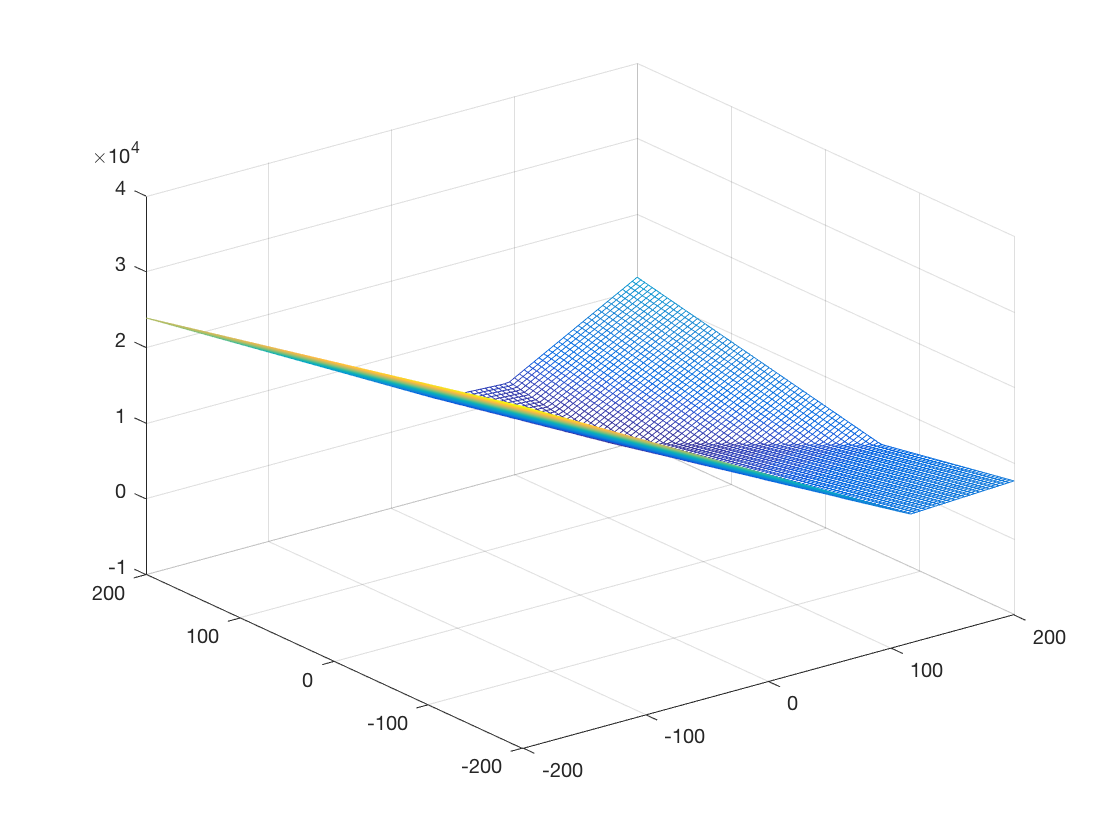
\includegraphics[width=.5\linewidth]{f5}
  \caption{3-D map for 2-D function}
  \label{f5}
\end{figure}

\subsubsection{$F_6$: Shifted Rosenbrock’s Function}

\begin{equation}
  F_6(x)=\sum_{i=1}^{D-1}{(100(z_i^2 - z_{i+1})^2 + (z_i - 1)^2)}
\end{equation}
\[ z=x-o+1 \]
\[ x \in [-100,100]^D \]

\begin{figure}[H]
  \centering
  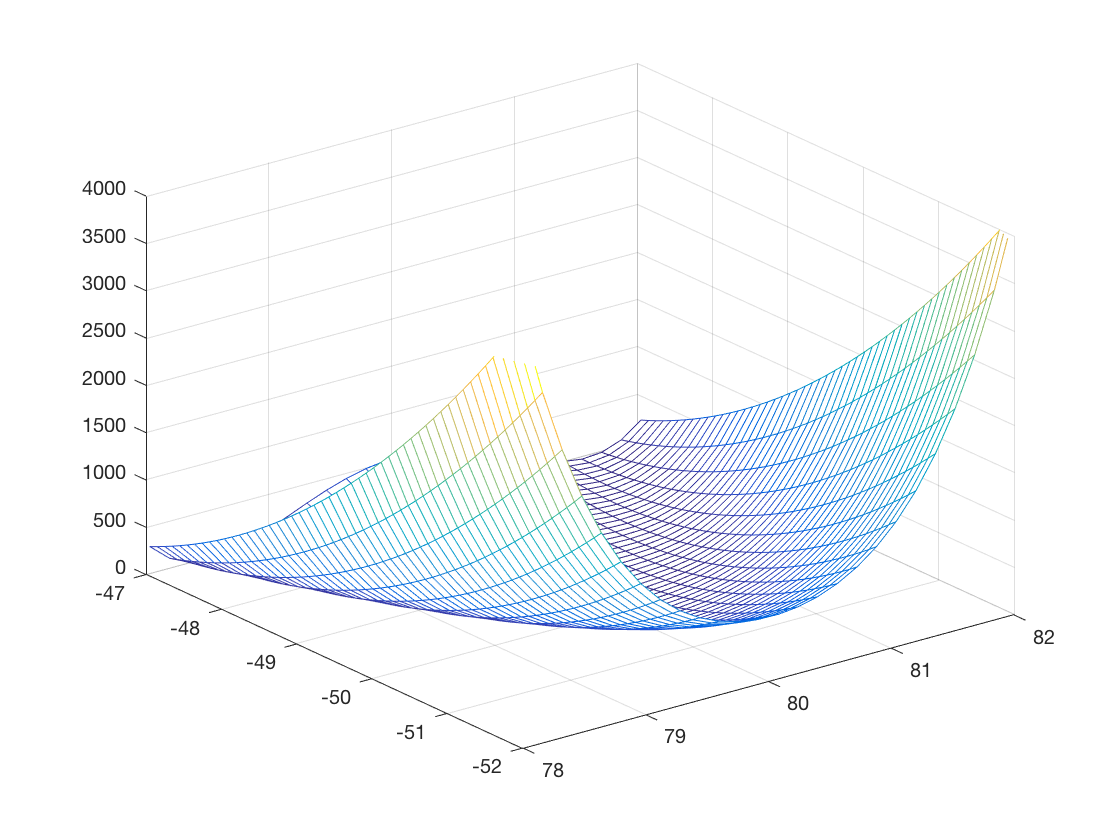
\includegraphics[width=.5\linewidth]{f6}
  \caption{3-D map for 2-D function}
  \label{f6}
\end{figure}

\subsubsection{$F_7$: Shifted Rotated Griewank’s Function without Bounds}

\begin{equation}
  F_7(x)=\sum_{i=1}^{D}{\frac{z_i^2}{4000}}-\prod_{i=1}^{D}{\cos{\frac{z_i}{\sqrt{i}}}}+1
\end{equation}
\[ z=(x-o)*M \]
\[ x \in [0,600]^D \]

\begin{figure}[H]
  \centering
  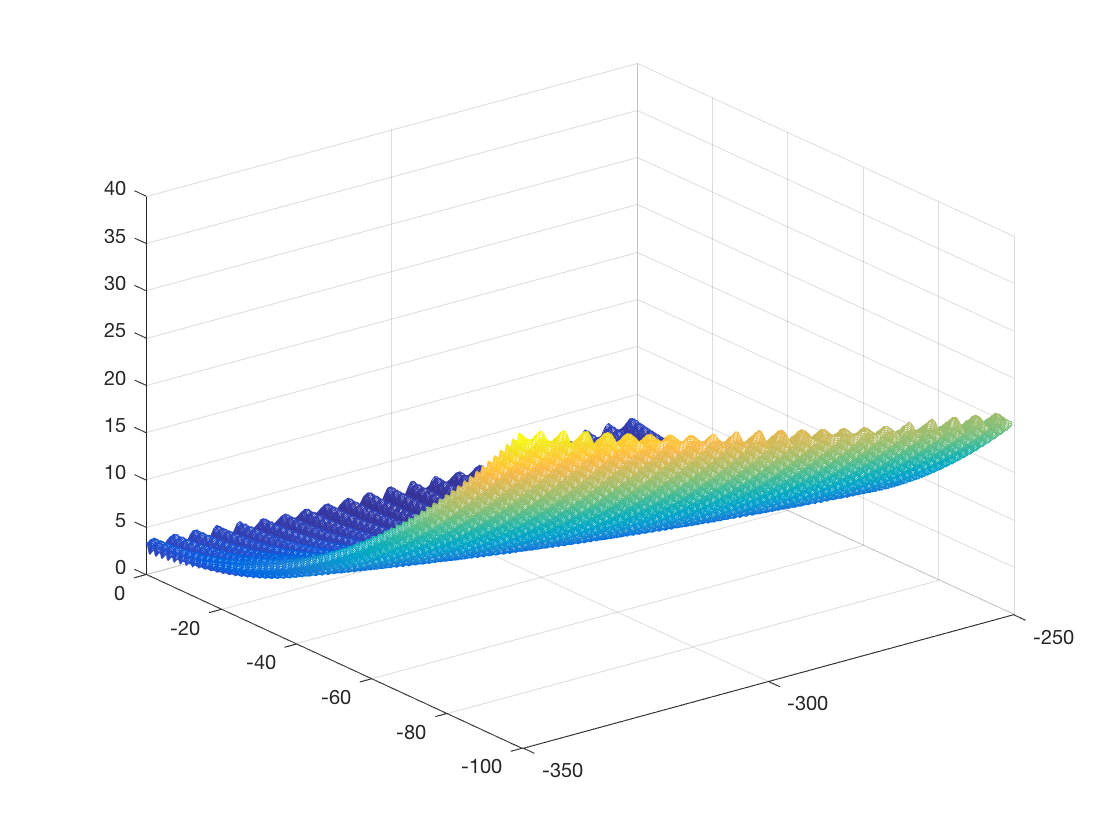
\includegraphics[width=.5\linewidth]{f7}
  \caption{3-D map for 2-D function}
  \label{f7}
\end{figure}

\subsubsection{$F_8$: Shifted Rotated Ackley’s Function with Global Optimum on Bounds}

\begin{equation}
  F_8(x)=-20\exp{(-0.2\sqrt{\frac{1}{D}\sum_{i=1}^{D}{z_i^2}})}-\exp{(\frac{1}{D}\sum_{i=1}^{D}{\cos{(2\pi z_i)}})} + 20 + e
\end{equation}
\[ z=(x-o)*M \]
\[ x \in [-32,32]^D \]

\begin{figure}[H]
  \centering
  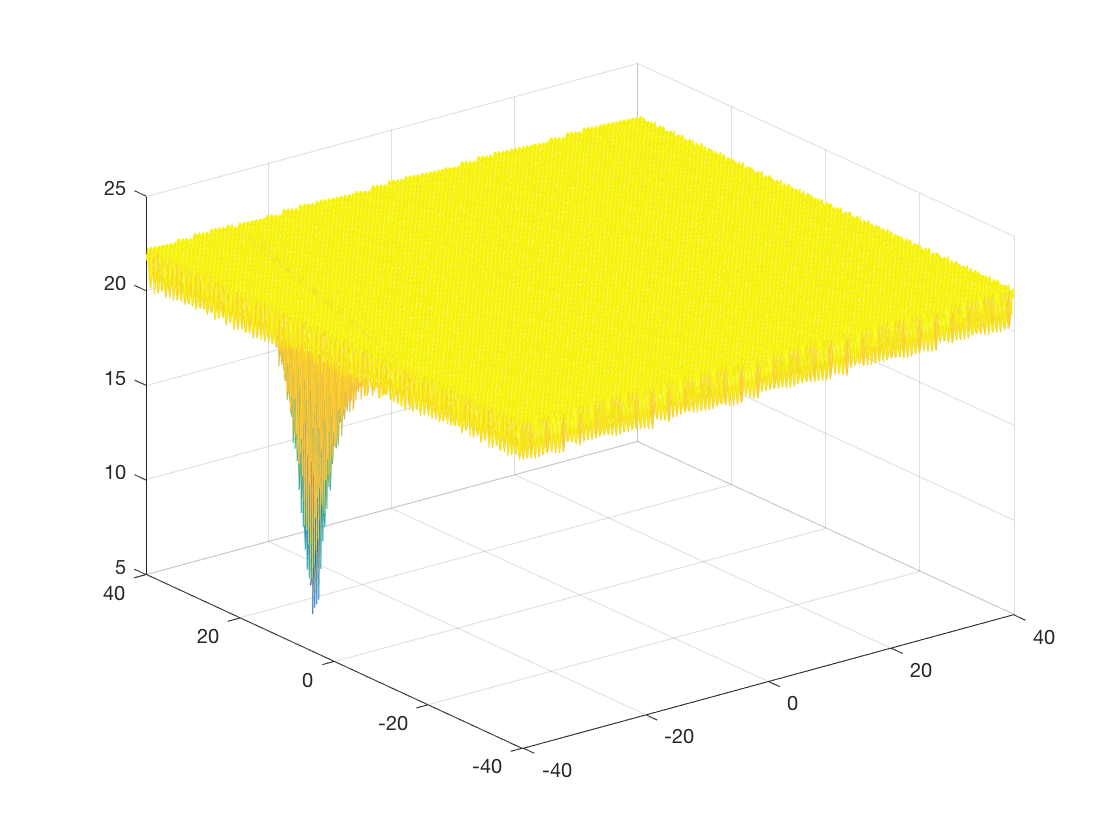
\includegraphics[width=.5\linewidth]{f8}
  \caption{3-D map for 2-D function}
  \label{f8}
\end{figure}

\subsubsection{$F_9$: Shifted Rastrigin’s Function}

\begin{equation}
  F_9(x)=\sum_{i=1}^{D}{z_i^2 - 10\cos{(2\pi z_i)} + 10}
\end{equation}
\[ z=x-o \]
\[ x \in [-5,5]^D \]

\begin{figure}[H]
  \centering
  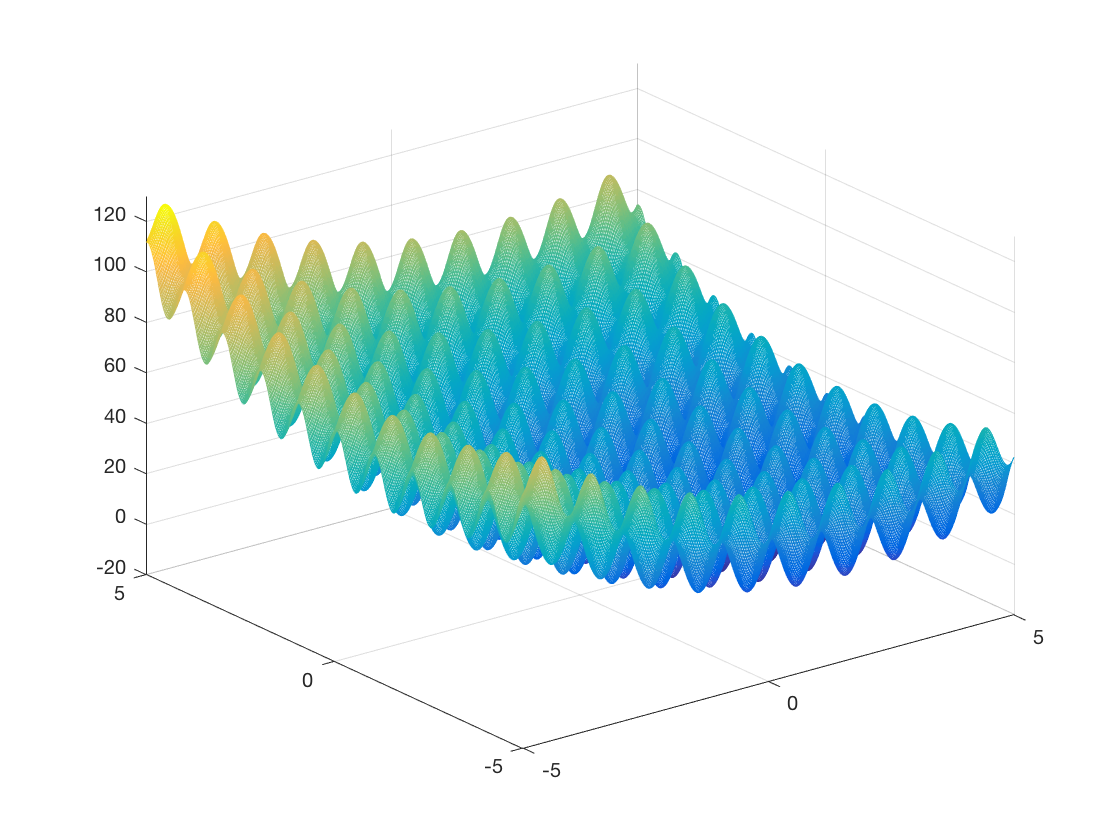
\includegraphics[width=.5\linewidth]{f9}
  \caption{3-D map for 2-D function}
  \label{f9}
\end{figure}

\subsubsection{$F_{10}$: Shifted Rotated Rastrigin’s Function}

\begin{equation}
  F_{10}(x)=\sum_{i=1}^{D}{z_i^2 - 10\cos{(2\pi z_i)} + 10}
\end{equation}
\[ z=(x-o)*M \]
\[ x \in [-5,5]^D \]

\begin{figure}[H]
  \centering
  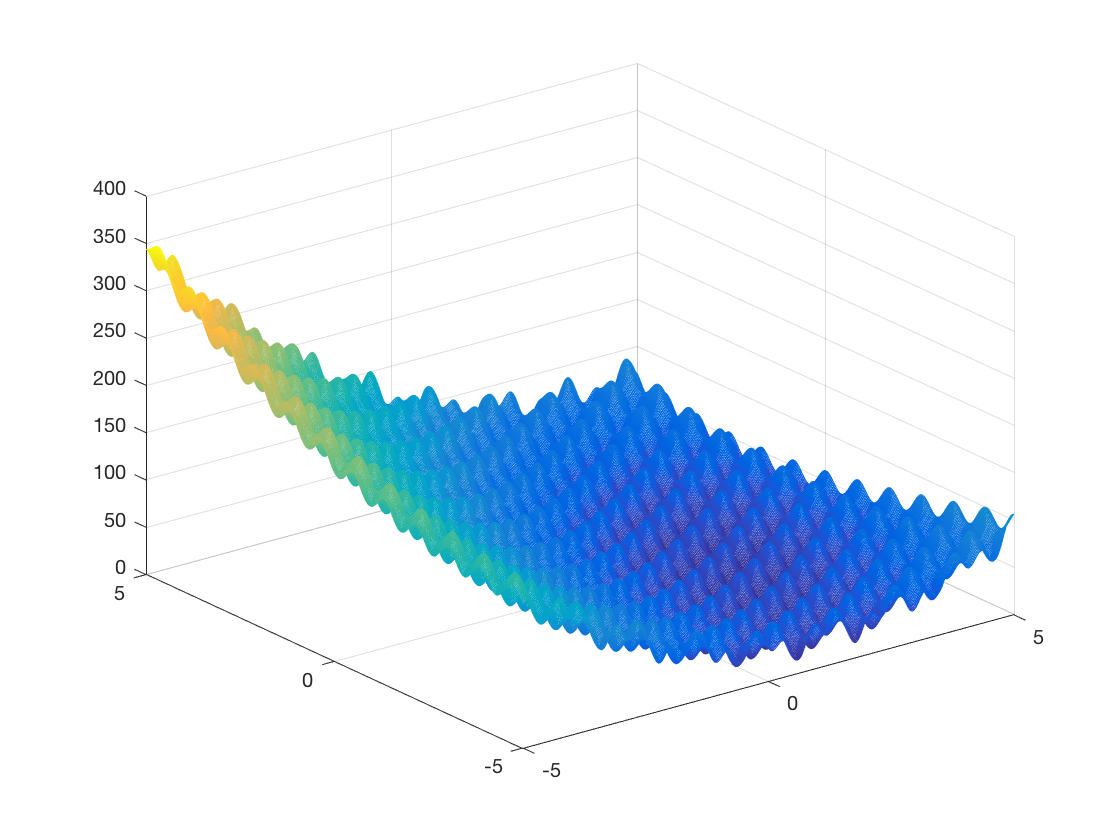
\includegraphics[width=.5\linewidth]{f10}
  \caption{3-D map for 2-D function}
  \label{f10}
\end{figure}

\subsection{Machine learning problem set}

To evaluate the optimization algorithms further I set have set out to apply them on a variety of machine learning problems. These will predominantly be applications of feed-forward neural networks (FFNN).

\subsubsection{$ML_{1}$: Training FFNNs to do function approximation}

The optimization algorithm were used to train FFNNs to perform function approximation and curve-fitting on seven sample data-sets which are available in Matlab's Neural Network Toolbox. The data-sets used are the following

\begin{enumerate}
  \item simplefit\_dataset (Simple fitting dataset)
  \item abalone\_dataset (Abalone shell rings dataset)
  \item bodyfat\_dataset (Body fat percentage dataset)
  \item building\_dataset (Building energy dataset)
  \item chemical\_dataset (Chemical sensor dataset)
  \item cho\_dataset (Cholesterol dataset)
  \item engine\_dataset (Engine behavior dataset)
  \item house\_dataset (House value dataset)
\end{enumerate}

The data sets contain two matrices. One with sample input vectors to the neural network and one with the expected correct output vectors. The function which the optimization algorithm directly optimize is the sum of squared errors as defined by

\begin{equation}
  sse(x,t) = \frac{1}{2n} \sum_{i=1}^{n}{(y(x)-t)^2}
\end{equation}

where $x$ is the input vector to neural network $y$, $t$ is the correct expected output which $y(x)$ should produce and n is the length of vector $x$.

\subsubsection{$ML_{2}$: Training FFNNs to do classification}

The optimization algorithm were used to train FFNNs to perform classification tasks on eight sample data-sets which are available in Matlab's Neural Network Toolbox. The data-sets used are the following

\begin{enumerate}
  \item simpleclass\_dataset(Simple pattern recognition dataset)
  \item cancer\_dataset (Breast cancer dataset)
  \item crab\_dataset (Crab gender dataset)
  \item glass\_dataset (Glass chemical dataset)
  \item iris\_dataset (Iris flower dataset)
  \item thyroid\_dataset (Thyroid function dataset)
  \item wine\_dataset (Italian wines dataset)
\end{enumerate}

The evaluation procedure is the same as for $ML_{1}$.

\subsubsection{$ML_{3}$: Training FFNNs to do clustering}

The optimization algorithm were used to train FFNNs to perform clustering tasks on one sample data-sets which is available in Matlab's Neural Network Toolbox. The data-sets used is the following

\begin{enumerate}
  \item simplecluster\_dataset (Simple clustering dataset)
\end{enumerate}

The evaluation procedure is the same as for $ML_{1}$ and $ML_{2}$.

\subsubsection{$ML_{4}$: Training a FFNN to play a simple snake game}

A simple ``Snake'' game was designed for testing the evolutionary algorithms on neural networks as applied to games. The game takes it's width and height as input parameters and constructs a square-grid which the snake will be able to move in. The snake is initialized to the center of the grid and is able to move left, right, up and down. A food square is initialized to a random square and replaced with a new random food square when it is consumed by the snake. After consuming a food square the snake gain an additional tail square. The snake dies if it runs into the edge of the grid or into itself.

The neural network controlling the snake takes a 12-dimensional representation of the snake, food and playing field and outputs a 4-dimensional vector which helps the snake decide in which direction it should move next.

Once the snake dies and the game is over a fitness score will be returned to the optimizing algorithm. The score is combination of how long the snake managed to live and how much food it ate. It is described by the equation below:

\begin{equation}
  fitness = food^{1.5} +  \frac{1}{1-e^{-lifetime}}  - 0.5
\end{equation}

The equation was constructed to force the snake to first learn how to survive but then not rely on moving in circles instead of looking for food.
